\documentclass[a4paper,12pt]{extarticle}
\usepackage[utf8x]{inputenc}
\usepackage[T1,T2A]{fontenc}
\usepackage[russian]{babel}
\usepackage{hyperref}
\usepackage{indentfirst}
\usepackage{listings}
\usepackage{color}
\usepackage{here}
\usepackage{array}
\usepackage{multirow}
\usepackage{graphicx}
\usepackage{amsmath}
\usepackage{amssymb}

\usepackage{caption}
\renewcommand{\lstlistingname}{Программа} % заголовок листингов кода

\bibliographystyle{ugost2008ls}

\usepackage{listings}
\lstset{ %
extendedchars=\true,
keepspaces=true,
language=C,						% choose the language of the code
basicstyle=\footnotesize,		% the size of the fonts that are used for the code
numbers=left,					% where to put the line-numbers
numberstyle=\footnotesize,		% the size of the fonts that are used for the line-numbers
stepnumber=1,					% the step between two line-numbers. If it is 1 each line will be numbered
numbersep=5pt,					% how far the line-numbers are from the code
backgroundcolor=\color{white},	% choose the background color. You must add \usepackage{color}
showspaces=false				% show spaces adding particular underscores
showstringspaces=false,			% underline spaces within strings
showtabs=false,					% show tabs within strings adding particular underscores
frame=single,           		% adds a frame around the code
tabsize=2,						% sets default tabsize to 2 spaces
captionpos=t,					% sets the caption-position to top
breaklines=true,				% sets automatic line breaking
breakatwhitespace=false,		% sets if automatic breaks should only happen at whitespace
escapeinside={\%*}{*)},			% if you want to add a comment within your code
postbreak=\raisebox{0ex}[0ex][0ex]{\ensuremath{\color{red}\hookrightarrow\space}},
texcl=true,
inputpath=listings,                     % директория с листингами
}

\usepackage[left=2cm,right=2cm,
top=2cm,bottom=2cm,bindingoffset=0cm]{geometry}

%% Нумерация картинок по секциям
\usepackage{chngcntr}
\counterwithin{figure}{subsection}
\counterwithin{table}{section}

%%Точки нумерации заголовков
\usepackage{titlesec}
\titlelabel{\thetitle.\quad}
\usepackage[dotinlabels]{titletoc}

%% Оформления подписи рисунка
\addto\captionsrussian{\renewcommand{\figurename}{Рис.}}
\captionsetup[figure]{labelsep = period}

%% Подпись таблицы
\DeclareCaptionFormat{hfillstart}{\hfill#1#2#3\par}
\captionsetup[table]{format=hfillstart,labelsep=newline,justification=centering,skip=-10pt,textfont=bf}

%% Путь к каталогу с рисунками
\graphicspath{{fig/}}

\begin{document}	% начало документа

% Титульная страница
\begin{titlepage}	% начало титульной страницы

	\begin{center}		% выравнивание по центру

		\large Санкт-Петербургский Политехнический Университет Петра Великого\\
		\large Институт компьютерных наук и технологий \\
		\large Кафедра компьютерных систем и программных технологий\\[6cm]
		% название института, затем отступ 6см
		
		\huge Телекоммуникационные технологии\\[0.5cm] % название работы, затем отступ 0,5см
		\large Отчет по лабораторной работе №3\\[0.1cm]
		\large Линейная фильтрация\\[5cm]

	\end{center}


	\begin{flushright} % выравнивание по правому краю
		\begin{minipage}{0.25\textwidth} % врезка в половину ширины текста
			\begin{flushleft} % выровнять её содержимое по левому краю

				\large\textbf{Работу выполнил:}\\
				\large Беседин Д.С.\\
				\large {Группа:} 33501/3\\
				
				\large \textbf{Преподаватель:}\\
				\large Богач Н.В.

			\end{flushleft}
		\end{minipage}
	\end{flushright}
	
	\vfill % заполнить всё доступное ниже пространство

	\begin{center}
	\large Санкт-Петербург\\
	\large \the\year % вывести дату
	\end{center} % закончить выравнивание по центру

\thispagestyle{empty} % не нумеровать страницу
\end{titlepage} % конец титульной страницы

\vfill % заполнить всё доступное ниже пространство

% Содержание
% Содержание
\renewcommand\contentsname{\centerline{Содержание}}
\tableofcontents
\newpage


\section{Цель работы}
Целью данной работы является приобретение навыков генерации и визуализации простых сигналов в среде MatLab, а также разложение этих сигналов в ряд Фурье для построения спектра сигналов.

\section{Постановка задачи}
Задачей работы является промоделировать сигналы в командном окне MATLAB и в среде Simulink из Главы 3, сс. 150–170 справочного пособия и получить их разложение в ряд Фурье.

\section{Теоретическая информация}
\subsection{Понятие сигналов как векторов отсчетов функций}
Аналоговый сигнал, с математической точки зрения, представляет собой функцию. Поэтому в среде  MatLab может быть удобно представлен как вектор дискретных отсчетов этой функции, а затем отобразить в виде графика зависимости значений этого вектора от значений вектора отсчетов времени. Второй вектор удобно формировать как возрастающую последовательность чисел, шаг между которыми есть величина, обратная частоте дискретизации.

Таким образом, определив вектор отсчетов времени и некоторые константы, необходимые для представления вида сигнала в математической формуле, такие как амплитуда колебаний, частота колебаний и так далее, мы может задать вектор значений функции в известных нам моментах времени для дальнейшего построения графика. Делается это путем использования известных математических законов и встроенных в MatLab функций генерации специальных сигналов.

\subsection{Затухающие сигналы}
Затухание обычного гармонического сигнала получается путем его домножения на убывающую экспоненциальную функцию, как показано ниже на \ref{pic:theor1}:
\begin{figure}[H]
	\begin{center}
		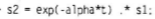
\includegraphics[scale=0.7]{theor1}
		\caption{Домножение сигнала на экспоненту в МатЛаб} 
		\label{pic:theor1} % название для ссылок внутри кода
	\end{center}
\end{figure}

\subsection{Одиночные импульсы}
Встроенная функция rectpuls работает по следующему принципу:
\begin{figure}[H]
	\begin{center}
		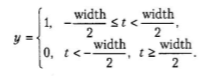
\includegraphics[scale=0.7]{theor4}
		\caption{Генерация прямоугольного импульса} 
		\label{pic:theor4} % название для ссылок внутри кода
	\end{center}
\end{figure}
где y-возвразаемое значение, t-вектор значений времени, сгенерированный заранее, width-ширин (длительность) импульса.

Встроенная функция tripuls работает по следующему принципу:
\begin{figure}[H]
	\begin{center}
		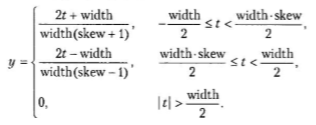
\includegraphics[scale=0.7]{theor5}
		\caption{Генерация треугольного импульса} 
		\label{pic:theor5} % название для ссылок внутри кода
	\end{center}
\end{figure}
где параметр skew - коэффициент ассимметрии импульса (по-умолчанию равен 0), а другие параметры имеют те же значения.

\subsection{Ограниченная полоса частот}
Для формирование сигнала, имещего ограниченный спектр, используется функция sinc:
\begin{figure}[H]
	\begin{center}
		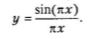
\includegraphics[scale=0.7]{theor6}
		\caption{Sinc} 
		\label{pic:theor6} % название для ссылок внутри кода
	\end{center}
\end{figure}
Спектральная функция сигнала в этом случае имеет прямоугольный вид:
\begin{figure}[H]
	\begin{center}
		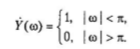
\includegraphics[scale=0.7]{theor6_1}
		\caption{Спектр Sinc'a} 
		\label{pic:theor6_1} % название для ссылок внутри кода
	\end{center}
\end{figure}

\subsection{Гауссов радиоимпульс}
Функция для получение отсчетов радиоимпульса имеет фнутри себя следую математичскию формулу:
\begin{figure}[H]
	\begin{center}
		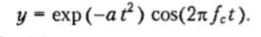
\includegraphics[scale=0.7]{theor7_1}
		\caption{Гауссов радиоимпульс} 
		\label{pic:theor7_1} % название для ссылок внутри кода
	\end{center}
\end{figure}
А спектр такого сигнала можно получить путем рпеобразования Фурье, формула которого представлена на \ref{pic:theor7_2} ниже:
\begin{figure}[H]
	\begin{center}
		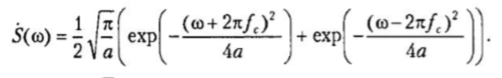
\includegraphics[scale=0.7]{theor7_2}
		\caption{Формула для разложения радиоимпульса} 
		\label{pic:theor7_2} % название для ссылок внутри кода
	\end{center}
\end{figure}

\subsection{Дирихле}
Функция Дирихле описывается формулой:
\begin{figure}[H]
	\begin{center}
		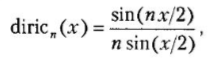
\includegraphics[scale=0.7]{theor10_1}
		\caption{Функция Дирихле} 
		\label{pic:theor10_1} % название для ссылок внутри кода
	\end{center}
\end{figure}
где n - целое положительное число.

Функцию Дирихле еще называют периодический sinc функцией.
При нечетном / четном значении параметра n функция приобретает вид:
\begin{figure}[H]
	\begin{center}
		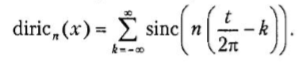
\includegraphics[scale=0.7]{theor10_2}
		\caption{Функция Дирихле при нечетном n} 
		\label{pic:theor10_2} % название для ссылок внутри кода
	\end{center}
\end{figure}
\begin{figure}[H]
	\begin{center}
		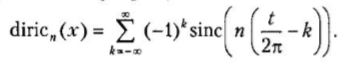
\includegraphics[scale=0.7]{theor10_3}
		\caption{Функция Дирихле при четном n} 
		\label{pic:theor10_3} % название для ссылок внутри кода
	\end{center}
\end{figure}

\subsection{Математические законы изменения мгновенной частоты}
В данной работе рассматриваются 3 закона - линейный, квадратичный и логарифмический. Формулы этих законов представлены на \ref{pic:theor11_1} - \ref{pic:theor11_3}:
\begin{figure}[H]
	\begin{center}
		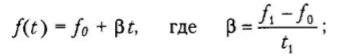
\includegraphics[scale=0.7]{theor11_1}
		\caption{Линейный закон} 
		\label{pic:theor11_1} % название для ссылок внутри кода
	\end{center}
\end{figure}
\begin{figure}[H]
	\begin{center}
		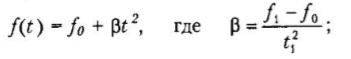
\includegraphics[scale=0.7]{theor11_2}
		\caption{Квадратичный закон} 
		\label{pic:theor11_2} % название для ссылок внутри кода
	\end{center}
\end{figure}
\begin{figure}[H]
	\begin{center}
		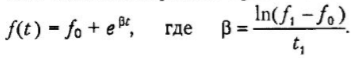
\includegraphics[scale=0.7]{theor11_3}
		\caption{Логарифмический закон} 
		\label{pic:theor11_3} % название для ссылок внутри кода
	\end{center}
\end{figure}
Стоит отметить, что логарифмический закон противоречит своему названию, т.к. зависимость частоты от времени в нем экспоненциальная, а не логарифмическая.

\subsection{Преобразование Фурье}
Для нахождение спектра сигнала чаще всего применяют разложение функции в ряд Фурье, или же преобразование Фурье.
Формула прямого преобразования Фурье выглядит следующим образом:
\begin{figure}[H]
	\begin{center}
		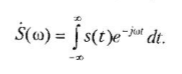
\includegraphics[scale=0.7]{theorFFT_1}
		\caption{Логарифмический закон} 
		\label{pic:theorFFT_1} % название для ссылок внутри кода
	\end{center}
\end{figure}



\section{Ход работы}

\subsection{Генерация затухающего гармонического сигнала}

\lstinputlisting[
	label=code:module1,
	caption={Код в МатЛаб},% для печати символ '_' требует выходной символ '\'
]{module1.m}
\parindent=1cm
Здесь представлен код программы, генерирующей затухающий сигнал и выводящий на экран 4 различных графика этого сигнала.

\begin{figure}[H]
	\begin{center}
		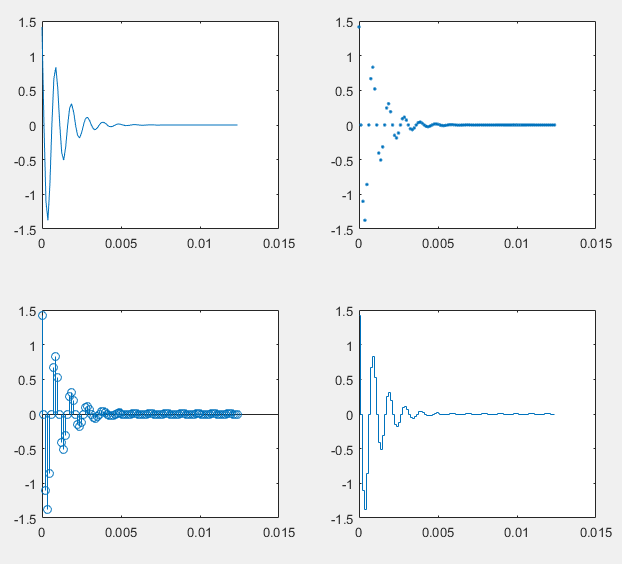
\includegraphics[scale=0.7]{graph1}
		\caption{Графики сигнала} 
		\label{pic:graph1} % название для ссылок внутри кода
	\end{center}
\end{figure}
На первом графике виден обычный вид затухающего гармонического сигнала, построенный средой МатЛаб по дискретным отсчетам. Второй график представляет из себя точки того же сигнала, соответствующие дискретным отсчетам. Третий график (stem) представляет собой те же точки, но в виде «лепестков» - как некоторые значения, отклоненные от нулевого. Четвертый график (stairs) — ступенчатый графк.

\begin{figure}[H]
	\begin{center}
		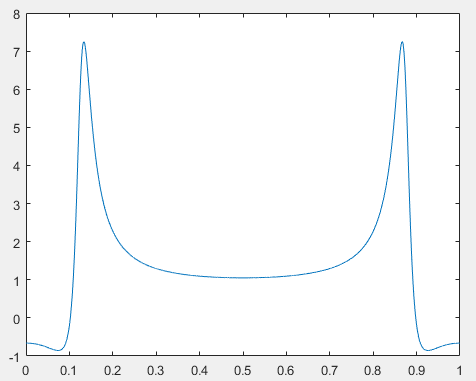
\includegraphics[scale=0.7]{spec1}
		\caption{Спектр сигнала} 
		\label{pic:spec1} % название для ссылок внутри кода
	\end{center}
\end{figure}
Спектр представленного выше сигнала получен с помощью разложение в ряд Фурье.

\subsection{Многоканальный сигнал}

\lstinputlisting[
	label=code:module2,
	caption={Код в МатЛаб},% для печати символ '_' требует выходной символ '\'
]{module2.m}
\parindent=1cm
Данный код генерирует сразу несколько сигналов, записываемых в одну матрицу, различающихся по частоте.

\begin{figure}[H]
	\begin{center}
		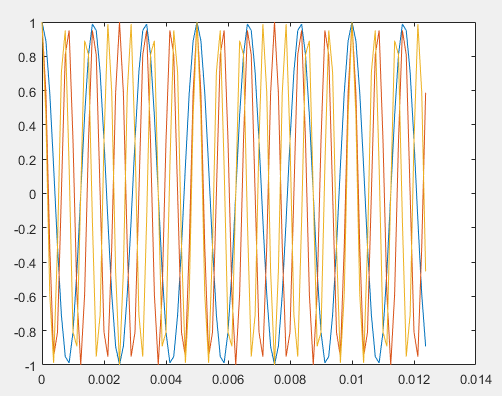
\includegraphics[scale=0.7]{graph2}
		\caption{График сигналов} 
		\label{pic:graph2} % название для ссылок внутри кода
	\end{center}
\end{figure}
На данном графике видно несколько гармонических сигналов, различающихся по частоте.

\begin{figure}[H]
	\begin{center}
		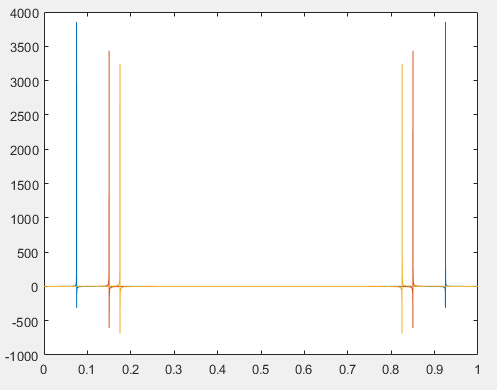
\includegraphics[scale=0.7]{spec2}
		\caption{Спектр сигналов} 
		\label{pic:spech2} % название для ссылок внутри кода
	\end{center}
\end{figure}
На этом рисунке видны спектры данных синусоид. Линии спектра сигнала с более высокой частотой распологаются ближе к нулю.

\subsection{Кусочные зависимости}

\lstinputlisting[
	label=code:module3,
	caption={Код в МатЛаб},% для печати символ '_' требует выходной символ '\'
]{module3.m}
\parindent=1cm
Данный участок кода генерирует и выводит на экран односторонний экспоненциальный импульс, прямоугольный импульс и несимметричный треугольный импульс согласно заданным уравнениям.

\begin{figure}[H]
	\begin{center}
		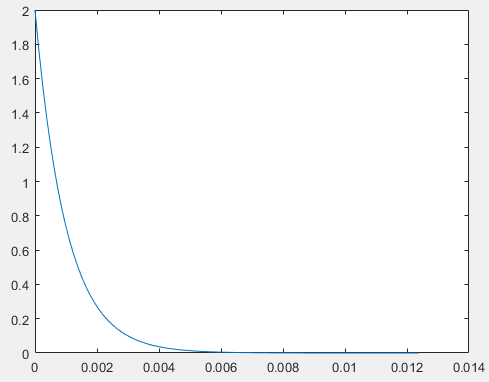
\includegraphics[scale=0.7]{graph3_1}
		\caption{Экспоненциальный импульс} 
		\label{pic:graph3_1} % название для ссылок внутри кода
	\end{center}
\end{figure}
\begin{figure}[H]
	\begin{center}
		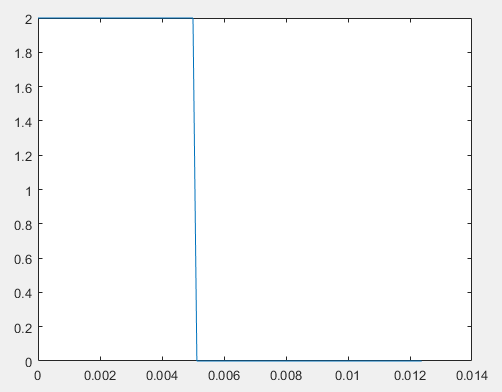
\includegraphics[scale=0.7]{graph3_2}
		\caption{Прямоугольный импульс} 
		\label{pic:graph3_2} % название для ссылок внутри кода
	\end{center}
\end{figure}
\begin{figure}[H]
	\begin{center}
		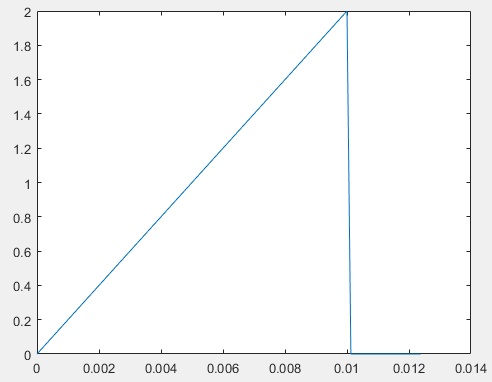
\includegraphics[scale=0.7]{graph3_3}
		\caption{Несимметричный треугольный импульс} 
		\label{pic:graph3_3} % название для ссылок внутри кода
	\end{center}
\end{figure}
На рисунках  \ref{pic:graph3_1} — \ref{pic:graph3_3} представлены графики сгенерированных сигналов, выведенных с помощью стандартной функции построения графиков в МатЛаб.

\begin{figure}[H]
	\begin{center}
		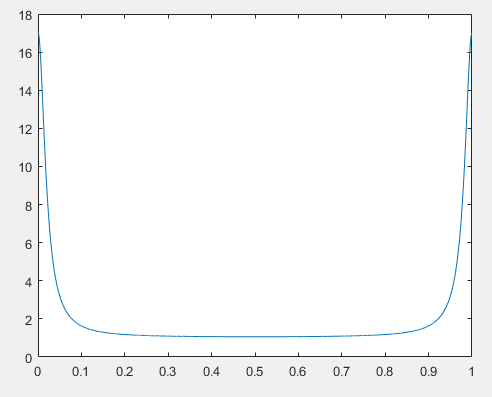
\includegraphics[scale=0.7]{spec3_1}
		\caption{Спектр экспоненциального импульса} 
		\label{pic:spec3_1} % название для ссылок внутри кода
	\end{center}
\end{figure}
\begin{figure}[H]
	\begin{center}
		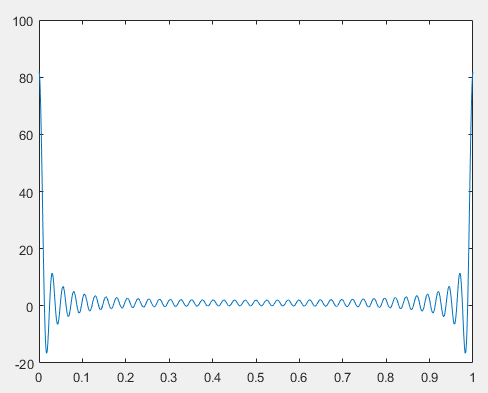
\includegraphics[scale=0.7]{spec3_2}
		\caption{Спектр прямоугольного импульса} 
		\label{pic:spec3_2} % название для ссылок внутри кода
	\end{center}
\end{figure}
\begin{figure}[H]
	\begin{center}
		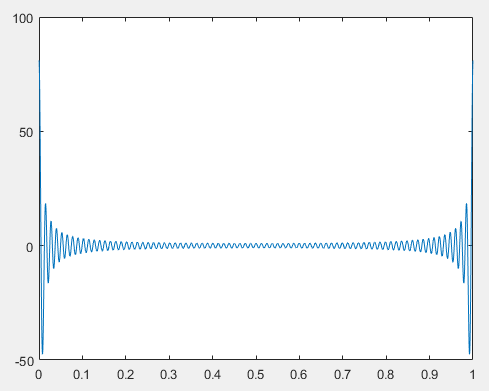
\includegraphics[scale=0.7]{spec3_3}
		\caption{спектр несимметричного треугольного импульса} 
		\label{pic:spec3_3} % название для ссылок внутри кода
	\end{center}
\end{figure}
На рисунках  \ref{pic:spec3_1} — \ref{pic:spec3_3} представлены спектры сигналов \ref{pic:graph3_1} — \ref{pic:graph3_3}.

\subsection{Прямоугольный импульс}

\lstinputlisting[
	label=code:module5,
	caption={Код в МатЛаб},% для печати символ '_' требует выходной символ '\'
]{module5.m}
\parindent=1cm
Данный сигнал генерируется путем соединения двух прямоугольных импульсов, с использованием встроенных функций.

\begin{figure}[H]
	\begin{center}
		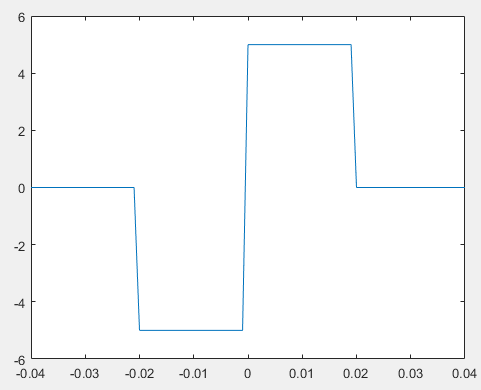
\includegraphics[scale=0.7]{graph4}
		\caption{Прямоугольные импульсы} 
		\label{pic:graph4} % название для ссылок внутри кода
	\end{center}
\end{figure}
На данном рисунке представлен график прямоугольных импульсов.

\begin{figure}[H]
	\begin{center}
		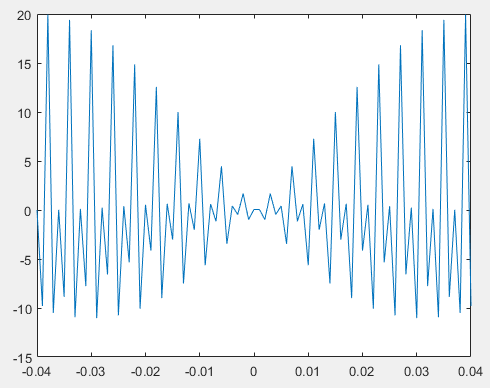
\includegraphics[scale=0.7]{spec4}
		\caption{Спектр прямоугольных импульсов} 
		\label{pic:spec4} % название для ссылок внутри кода
	\end{center}
\end{figure}
Спектр прямоугольного импульса получен как разложение сигнала в ряд Фурье.

\subsection{Трапецевидный импульс}

\lstinputlisting[
	label=code:module6,
	caption={Код в МатЛаб},% для печати символ '_' требует выходной символ '\'
]{module6.m}
\parindent=1cm
Данный сигнал генерируется разностью двух треугольных импульсов, с использованием встроенной функции tripuls.

\begin{figure}[H]
	\begin{center}
		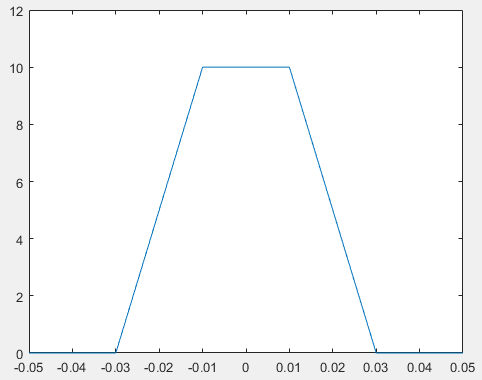
\includegraphics[scale=0.7]{graph5}
		\caption{Трапецевидный импульс} 
		\label{pic:graph5} % название для ссылок внутри кода
	\end{center}
\end{figure}
На данном рисунке представлен вид трапецевидного импульса в среде МатЛаб.

\begin{figure}[H]
	\begin{center}
		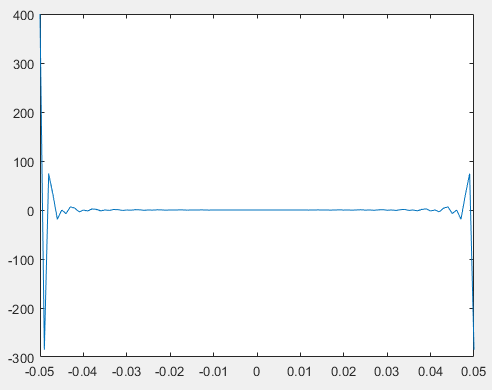
\includegraphics[scale=0.7]{spec5}
		\caption{Спектр трапецевидного импульса} 
		\label{pic:spec5} % название для ссылок внутри кода
	\end{center}
\end{figure}
На рисунке представлен спектр трапецевидного импульса.

\subsection{Импульс с ограниченной полосой частот}

\lstinputlisting[
	label=code:module7,
	caption={Код в МатЛаб},% для печати символ '_' требует выходной символ '\'
]{module7.m}
\parindent=1cm
Данный код генерирует сигнал, у которого спектр ограничен по частоте. Затем выводится и сам спектр данного сигнала, что можно увидеть на рисунках ниже:

\begin{figure}[H]
	\begin{center}
		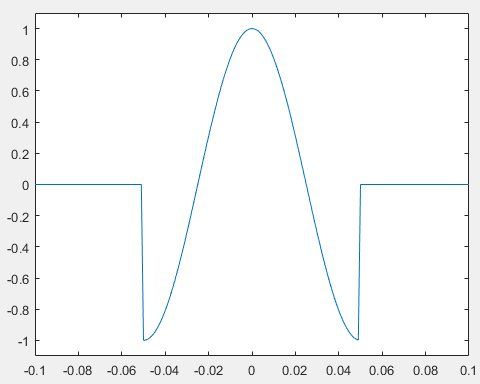
\includegraphics[scale=0.7]{graph6_1}
		\caption{Сигнал с ограниченным спектром} 
		\label{pic:graph6_1} % название для ссылок внутри кода
	\end{center}
\end{figure}
\begin{figure}[H]
	\begin{center}
		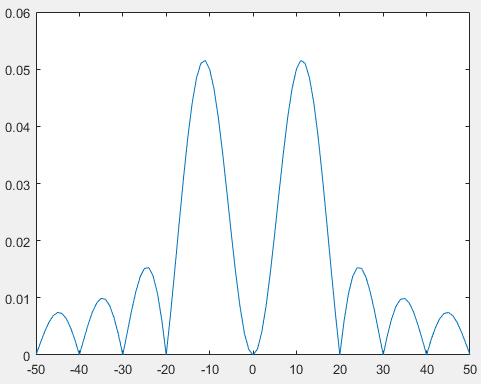
\includegraphics[scale=0.7]{graph6_2}
		\caption{Ограниченный спектр сигнала} 
		\label{pic:graph6_2} % название для ссылок внутри кода
	\end{center}
\end{figure}
Спектр сигнала получен с помощь функции sinc.

\subsection{Гауссов радиоимпульс}

\lstinputlisting[
	label=code:module8,
	caption={Код в МатЛаб},% для печати символ '_' требует выходной символ '\'
]{module8.m}
\parindent=1cm
Данный код генерирует Гауссов радиоимпульс с помощью встроенной функции gauspuls, а затем находит спектр этого сигнала, выражая его в дБ.

\begin{figure}[H]
	\begin{center}
		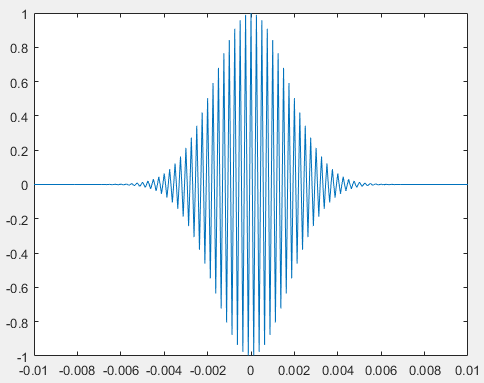
\includegraphics[scale=0.7]{graph7_1}
		\caption{Гауссов радиоимпульс} 
		\label{pic:graph7_1} % название для ссылок внутри кода
	\end{center}
\end{figure}
\begin{figure}[H]
	\begin{center}
		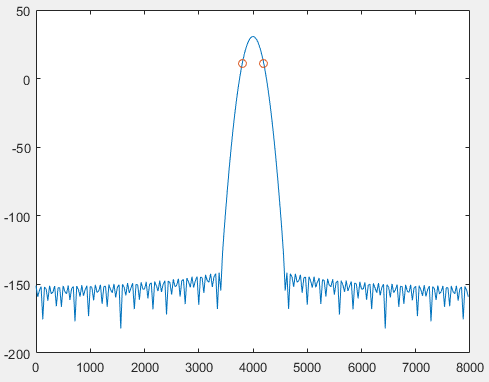
\includegraphics[scale=0.7]{graph7_2}
		\caption{Амплитудный спектр радиоимпульса} 
		\label{pic:graph7_2} % название для ссылок внутри кода
	\end{center}
\end{figure}
На графике спектра также отмечены расчетные границы этого спектра.

\subsection{Последовательности импульсов}

\lstinputlisting[
	label=code:module9,
	caption={Код в МатЛаб},% для печати символ '_' требует выходной символ '\'
]{module9.m}
\parindent=1cm
Данный код генерирует треугольные импульсы с заданными амплитудами, через заданные промежутки времени.

\begin{figure}[H]
	\begin{center}
		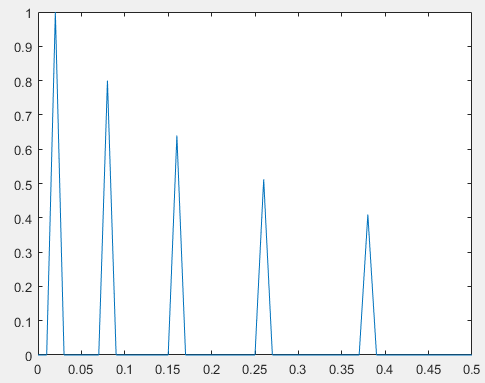
\includegraphics[scale=0.7]{graph8_1}
		\caption{Треугольные импульсы} 
		\label{pic:graph8_1} % название для ссылок внутри кода
	\end{center}
\end{figure}
\begin{figure}[H]
	\begin{center}
		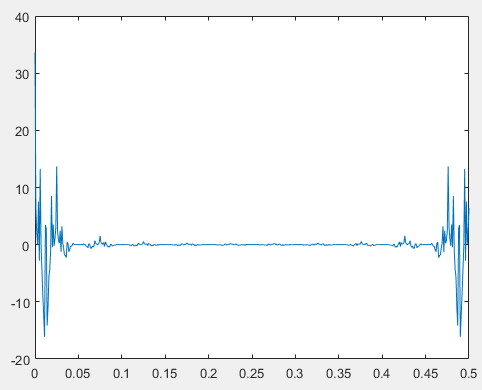
\includegraphics[scale=0.7]{spec8_1}
		\caption{Спектр импульсов} 
		\label{pic:spec8_1} % название для ссылок внутри кода
	\end{center}
\end{figure}
На рисунках представлены - треугольные импульсы, сгенерированные с помощью встроенной функции, (\ref{pic:graph8_1}) и спектр этого сигнала (\ref{pic:spec8_1}).

\lstinputlisting[
	label=code:module10,
	caption={Код в МатЛаб},% для печати символ '_' требует выходной символ '\'
]{module10.m}
\parindent=1cm
Данный код генерирует и выводит гармонические импульсы.

\begin{figure}[H]
	\begin{center}
		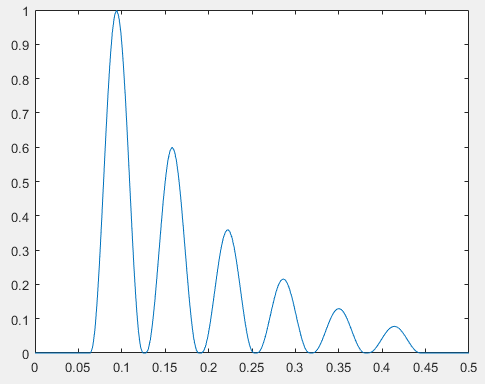
\includegraphics[scale=0.7]{graph8_2}
		\caption{Гармонические импульсы} 
		\label{pic:graph8_2} % название для ссылок внутри кода
	\end{center}
\end{figure}
Данные импульсы сгенерированы функцией pulstran из вектора отсчетов одиночного импульса.
\begin{figure}[H]
	\begin{center}
		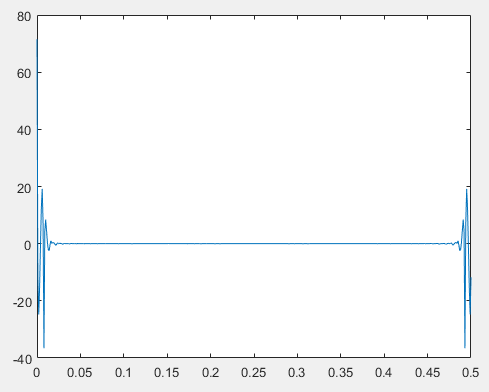
\includegraphics[scale=0.7]{spec8_2}
		\caption{Спектр гармонических импульсов} 
		\label{pic:spec8_2} % название для ссылок внутри кода
	\end{center}
\end{figure}
На рисунке представлен спектр гармонических импульсов.


\subsection{Генерация периодических сигналов}

\lstinputlisting[
	label=code:module11,
	caption={Код в МатЛаб},% для печати символ '_' требует выходной символ '\'
]{module11.m}
\parindent=1cm
Данная программа создает и выводит на экран периодически повторяющиеся прямоугольные сигналы, создаваемые с помощью функции square.

\begin{figure}[H]
	\begin{center}
		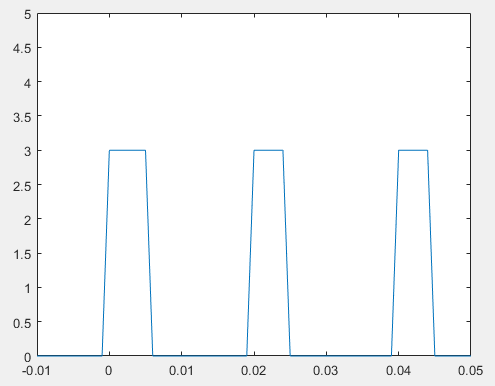
\includegraphics[scale=0.7]{graph9_1}
		\caption{Периодические прямоугольные импульсы} 
		\label{pic:graph9_1} % название для ссылок внутри кода
	\end{center}
\end{figure}
Импульсы обладают одинаковой длительностью и временем паузы между ними, что можно увидеть более отчетливо, если увеличить частоту дискретизации.
\begin{figure}[H]
	\begin{center}
		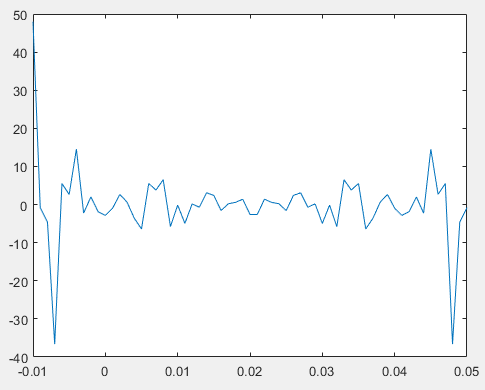
\includegraphics[scale=0.7]{spec9_1}
		\caption{Спектр прямоугольных импульсов} 
		\label{pic:spec9_1} % название для ссылок внутри кода
	\end{center}
\end{figure}

\lstinputlisting[
	label=code:module12,
	caption={Код в МатЛаб},% для печати символ '_' требует выходной символ '\'
]{module12.m}
\parindent=1cm
Эта программа, используя функцию sawtooth, создает импульсы треугольной формы с заданными параметрами.

\begin{figure}[H]
	\begin{center}
		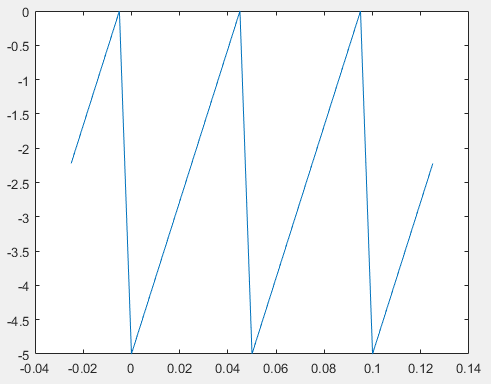
\includegraphics[scale=0.7]{graph9_2}
		\caption{Треугольные импульсы sawtooth} 
		\label{pic:graph9_2} % название для ссылок внутри кода
	\end{center}
\end{figure}
\begin{figure}[H]
	\begin{center}
		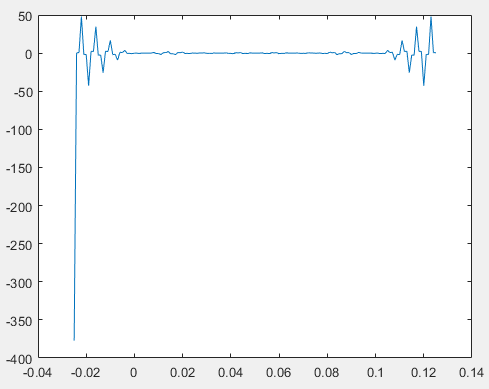
\includegraphics[scale=0.7]{spec9_2}
		\caption{Спектр прямоугольных импульсов} 
		\label{pic:spec9_2} % название для ссылок внутри кода
	\end{center}
\end{figure}

\subsection{Функция Дирихле}

\lstinputlisting[
	label=code:module13,
	caption={Код в МатЛаб},% для печати символ '_' требует выходной символ '\'
]{module13.m}
\parindent=1cm
Программа использует встроенную функцию diric для создания выборки из функции Дирихле с четным и нечетным значением параметра.

\begin{figure}[H]
	\begin{center}
		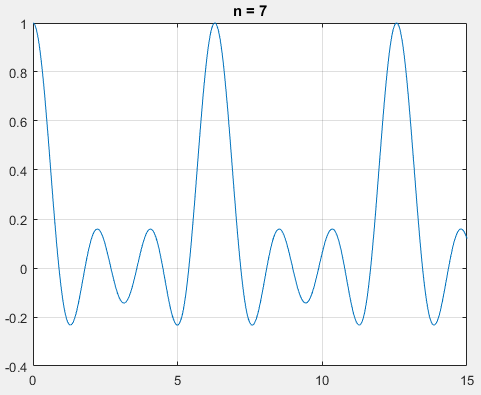
\includegraphics[scale=0.7]{graph10_1}
		\caption{Функция Дирихле с параметром равным 7} 
		\label{pic:graph10_1} % название для ссылок внутри кода
	\end{center}
\end{figure}
\begin{figure}[H]
	\begin{center}
		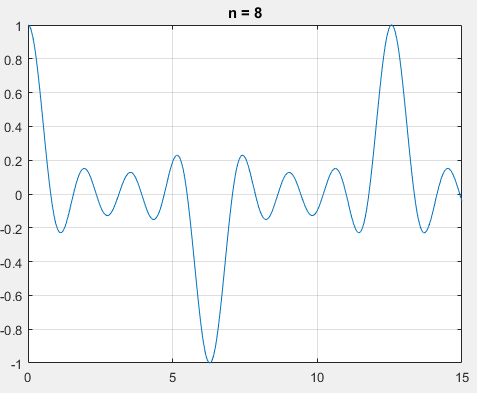
\includegraphics[scale=0.7]{graph10_2}
		\caption{Функция Дирихле с параметром равным 8} 
		\label{pic:graph10_2} % название для ссылок внутри кода
	\end{center}
\end{figure}
Видно, что нечетный параметр обеспечивает однонаправленные импульсы, а большее значение параметра увеличивает частоту колебаний.

\begin{figure}[H]
	\begin{center}
		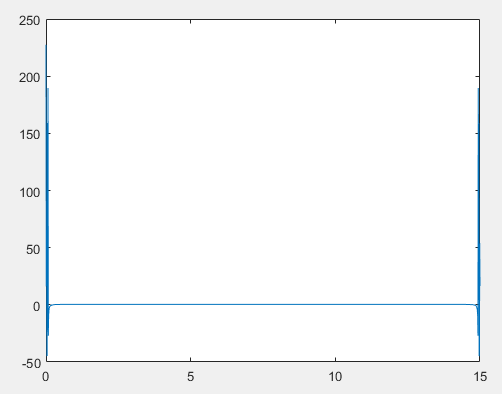
\includegraphics[scale=0.7]{spec10_1}
		\caption{Спектр функции Дирихле с параметром равным 7} 
		\label{pic:spec10_1} % название для ссылок внутри кода
	\end{center}
\end{figure}
\begin{figure}[H]
	\begin{center}
		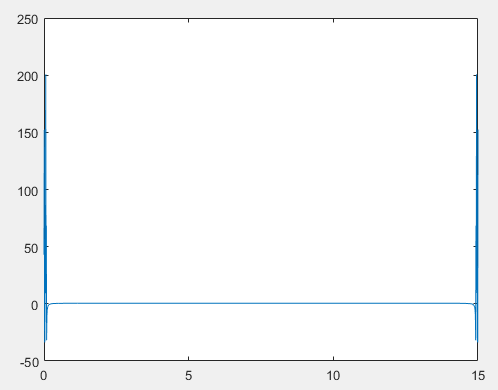
\includegraphics[scale=0.7]{spec10_2}
		\caption{Српектр функция Дирихле с параметром равным 8} 
		\label{pic:spec10_2} % название для ссылок внутри кода
	\end{center}
\end{figure}

\subsection{Сигнал с меняющейся частотой}

\lstinputlisting[
	label=code:module14,
	caption={Код в МатЛаб},% для печати символ '_' требует выходной символ '\'
]{module14.m}
\parindent=1cm
Эта программа с помощью функции chirp генерирует колебания, мгновенная частота которых изменяется согласно выбранной функции. В данном примере рассмотрены 3 таких функции — линейная, квадратичная и логарифмическая. На экран выводятся спектрограммы этих сигналов — зависимость мгновенного амплитудного спектра от времени.

\begin{figure}[H]
	\begin{center}
		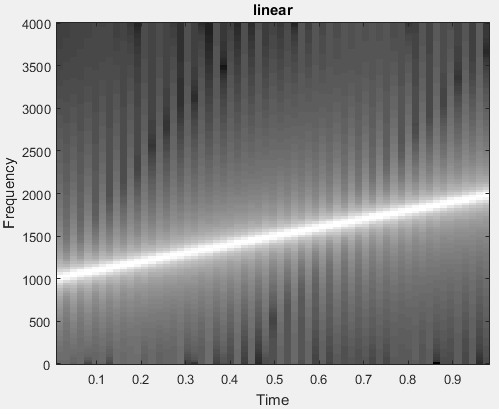
\includegraphics[scale=0.7]{graph11_1}
		\caption{Спектрограмма линейной функции chirp} 
		\label{pic:graph11_1} % название для ссылок внутри кода
	\end{center}
\end{figure}
\begin{figure}[H]
	\begin{center}
		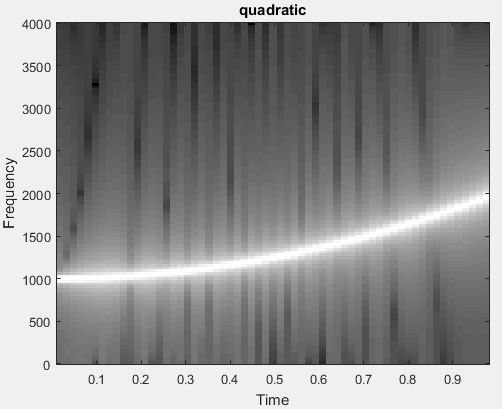
\includegraphics[scale=0.7]{graph11_2}
		\caption{Спектрограмма квадратичной функции chirp} 
		\label{pic:graph11_2} % название для ссылок внутри кода
	\end{center}
\end{figure}
\begin{figure}[H]
	\begin{center}
		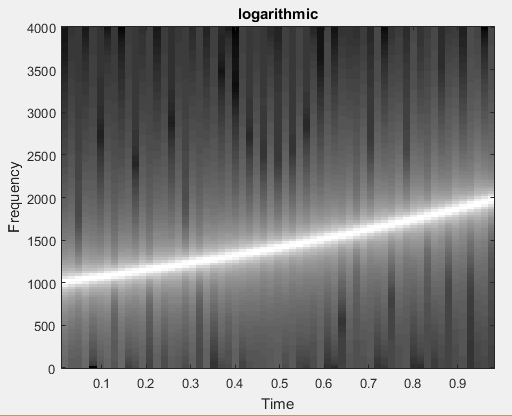
\includegraphics[scale=0.7]{graph11_3}
		\caption{Спектрограмма логарифмической функции chirp} 
		\label{pic:graph11_3} % название для ссылок внутри кода
	\end{center}
\end{figure}
На рисунках \ref{pic:graph11_2}, \ref{pic:graph11_2} и \ref{pic:graph11_3} показаны спектрограммы, наглядно демонстрирующие характер изменения мгновенной частоты сигнала.

\section{Выводы}

В данной работе исследованы методы генерации и визуализации различных сигналов в среде МатЛаб. 

Нами рассмотрены различные виды сигналов - детерминиированные сигналы, периодические, конечне (финитные) и бесконечные, гармонические колебания и сигналы, полученные на из основе, сигналы, представляюзие из себя единичные импульсы различной формы.

Полученыи построены спектры сигналов с помощью преобразования Фурье, встроенного в среду МатЛаб.
\end{document}

